\ifdefined\USERMANUAL
  \newcommand{\doctype}{BEDIENUNGSANLEITUNG}
\else
  \newcommand{\doctype}{REFERENZKARTEN}
\fi

\maketitlepage{TAIPO}{MIDI-Erweiterung}{TAIPO_SILVER_cutout_small_2}{\doctype}

\newpage
\tableofcontents
\newpage
\part{Übersicht}
\newpage
\section{Übersicht}\label{section:installation}
\subsection{Übersicht}
\paragraph*{}
Die \textbf{TAIPO} MIDI-Erweiterung ermöglicht eine nahtlose Verbindung von The Centre mit externen Geräten, einschließlich Computern, über ein standardmäßiges MIDI-TRS-Kabel Typ B.
\subsection{Lieferumfang}
\paragraph*{}
Das \textbf{TAIPO}-Paket enthält folgende Zubehörteile:
\begin{enumerate}
  \item \textbf{TAIPO} Eurorack-Modul
  \item Standard-Eurorack-Stromkabel (10-polig auf 16-polig)
  \item MIDI-EX-Verbindungskabel zur Anbindung an \textbf{The Centre}
\end{enumerate}

\newpage
\part{Installation}
\newpage
\section{Installation}
\subsection{Installationsschritte}
\paragraph*{}
Die Installation des \textbf{TAIPO}-Moduls folgt dem Standardverfahren für die Installation eines Eurorack-Moduls in Ihr Gehäuse.

\begin{figure}[h]
  \centering
  \includegraphics[height=0.5\linewidth]{taipo_the_centre_cable_install.jpg}
  \includegraphics[height=0.5\linewidth]{taipo_cable_install.jpg}
  \caption{Kabelinstallation an beiden Enden}
  \label{fig:midsinglenote}
\end{figure}

\subsection{Wichtige Hinweise zur Installation}
\paragraph*{}
Achten Sie bei der Installation auf die korrekte Ausrichtung des Kabels. Die Farbreihenfolge an der The Centre-Seite sollte von oben beginnend \textbf{SCHWARZ, ROT, GELB, GRÜN} sein, während sie an der TAIPO-Seite umgekehrt ist: \textbf{GRÜN, GELB, ROT, SCHWARZ}.
\newline$\blacksquare$ \textbf{Wichtig}: An der The Centre-Seite schließen Sie das Kabel wie in der obigen Abbildung gezeigt an den MIDI-EX-Anschluss an. Der zweite Anschluss dient zur Weiterleitung des MIDI-Ausgangs von The Centre an TWINS.

\newpage
\part{MIDI}
\newpage
\section{MIDI-Kabeltypen}
\subsection{TAIPO-Kabeltyp}
\paragraph*{}
Das \textbf{TAIPO} verwendet ein 3,5-mm-TRS-Kabel (Tip-Ring-Shield) Typ B. Siehe: \underline{\nameref{section:cabletypeb}}
\subsection{Über das MIDI-Signal}
\paragraph*{}
Das MIDI-Signal wird über ein MIDI-Kabel mit dem RS-232-Protokoll bei einer nicht standardmäßigen Geschwindigkeit von 31.250 Baud (Bits pro Sekunde) übertragen. MIDI-Verbindungen sind gerichtet, was bedeutet, dass die interne Pin-Konfiguration des Kabels entscheidend ist, da der Strom in eine Richtung fließt. Während standardmäßige MIDI-DIN-Kabel keine Probleme verursachen, können 3,5-mm-TRS-Kabel aufgrund des anfänglichen Fehlens eines einheitlichen Standards unterschiedlich verdrahtet sein, was zur Entstehung mehrerer Standards geführt hat.
\newline$\blacksquare$ \textbf{Hinweis}: Unterschiedliche TRS-Standards sind nicht austauschbar oder kompatibel. Zum Verbinden von Geräten mit unterschiedlichen TRS-Standards muss ein passendes Kabel verwendet werden.
\subsection{DIN-Anschluss}
Das standardmäßige MIDI-Kabel verwendet einen 5-poligen DIN-Anschluss für eine zuverlässige Verbindung.
\subsection{TRS-Anschlusstypen}
\subsubsection{Typ-A-Anschluss}
Der TRS-Typ A definiert den \textbf{TIP} des 3,5-mm-Steckers als \textit{\textbf{Quelle}} und den \textbf{RING} als \textit{\textbf{Senke}}.
\newline
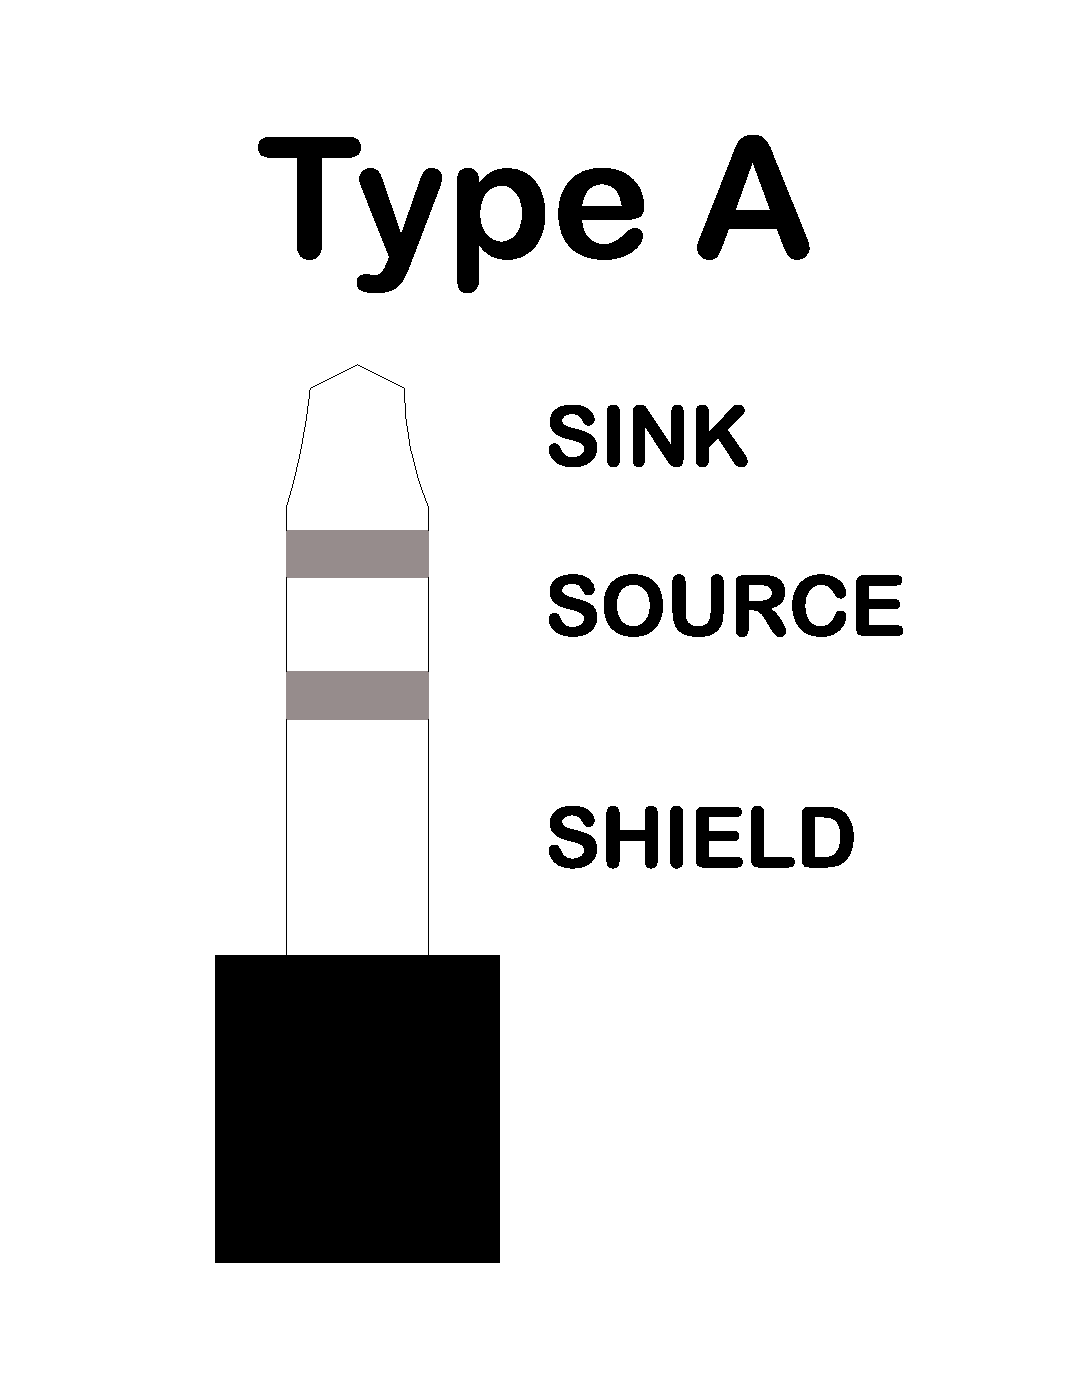
\includegraphics[height=0.3\linewidth]{midi_trs_type_a.eps}
\newline$\bigstar$ Marken, die Typ A verwenden: Korg, Akai
\subsubsection{Typ-B-Anschluss}\label{section:cabletypeb}
Der TRS-Typ B definiert den \textbf{TIP} des 3,5-mm-Steckers als \textit{\textbf{Senke}} und den \textbf{RING} als \textit{\textbf{Quelle}}.
\newline$\blacksquare$ Typ B ist in der Eurorack-Modular-Community weit verbreitet.
\newline
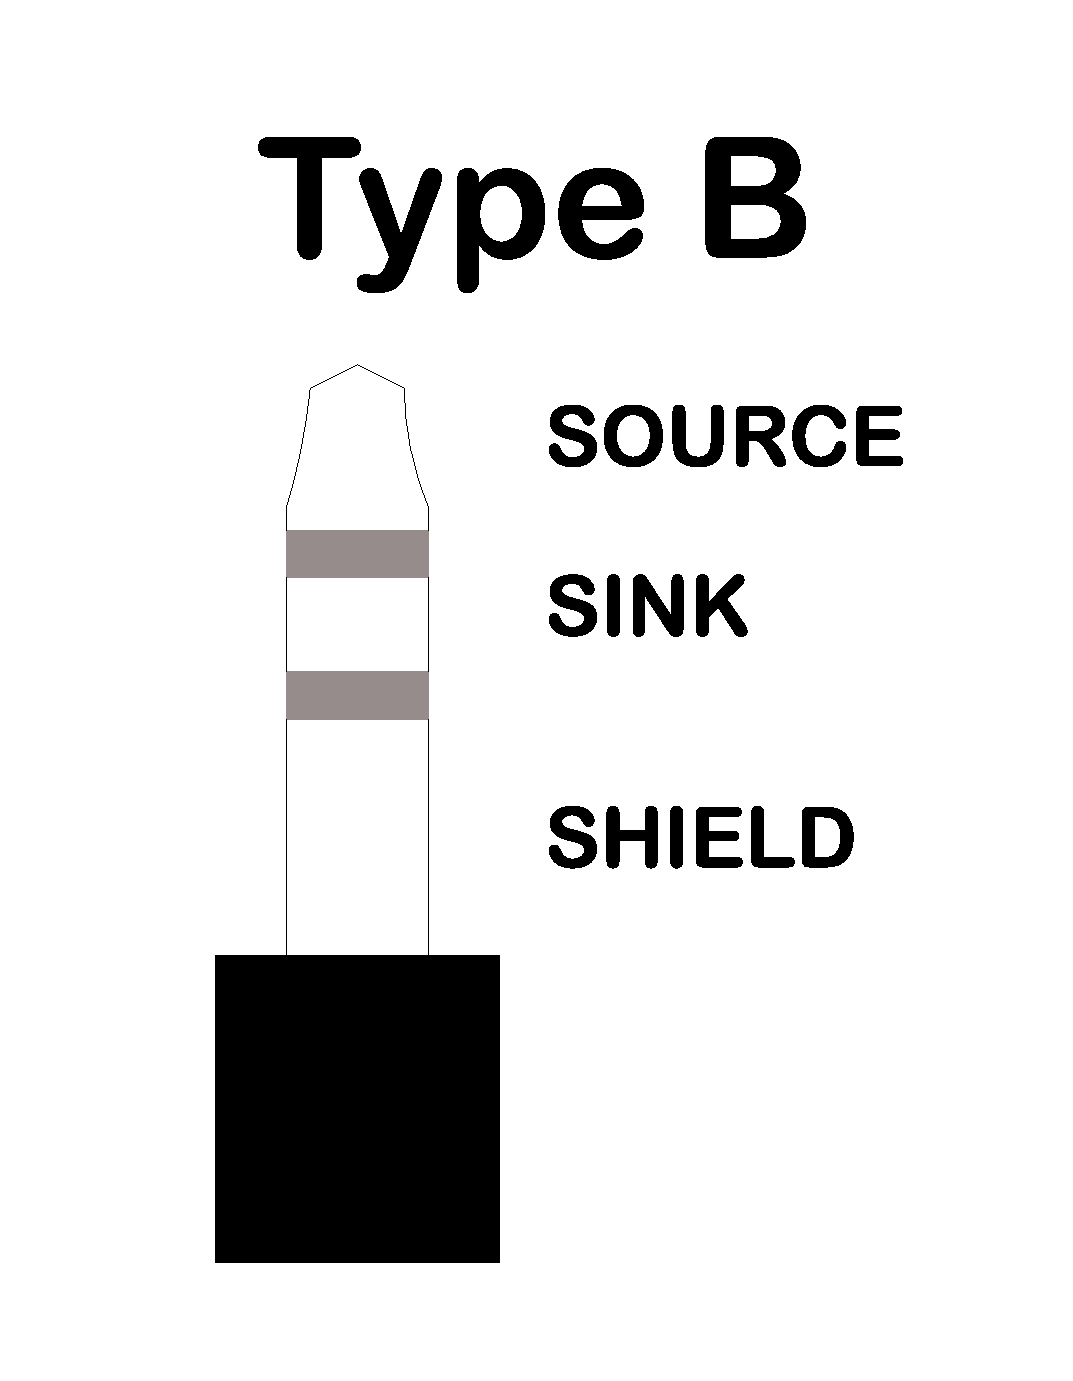
\includegraphics[height=0.3\linewidth]{midi_trs_type_b.eps}
\newline$\bigstar$ Marken, die Typ B verwenden: Arturia, Novation, 1010 Music